\documentclass[12pt,a4paper]{article}
\usepackage[utf8]{inputenc}
\usepackage{graphicx}
\usepackage{tikz}
\usetikzlibrary{fit}
\usepackage{lmodern}
\usepackage{sectsty}
\usepackage{hyperref}

\sectionfont{\color{cyan}}
\begin{document}
   \begin{titlepage}
      {\fontfamily{lmss}\selectfont
          \centering
          
\includegraphics[width=0.40\textwidth]{logo.png}\par\vspace{1cm}
          {\LARGE CSIR \par}
          \vspace{0.25cm}
          {\huge\bfseries \color{cyan}Electronically Timing Athletes\par}
          \vspace{1cm}
          {\Large\textit{by} Brute Force\par}
         \vspace{0.25cm}
         \begin{tikzpicture}
            \node [inner sep=0pt,,outer sep=0pt,clip,rounded corners=0.5cm] (pict) at (0,0) {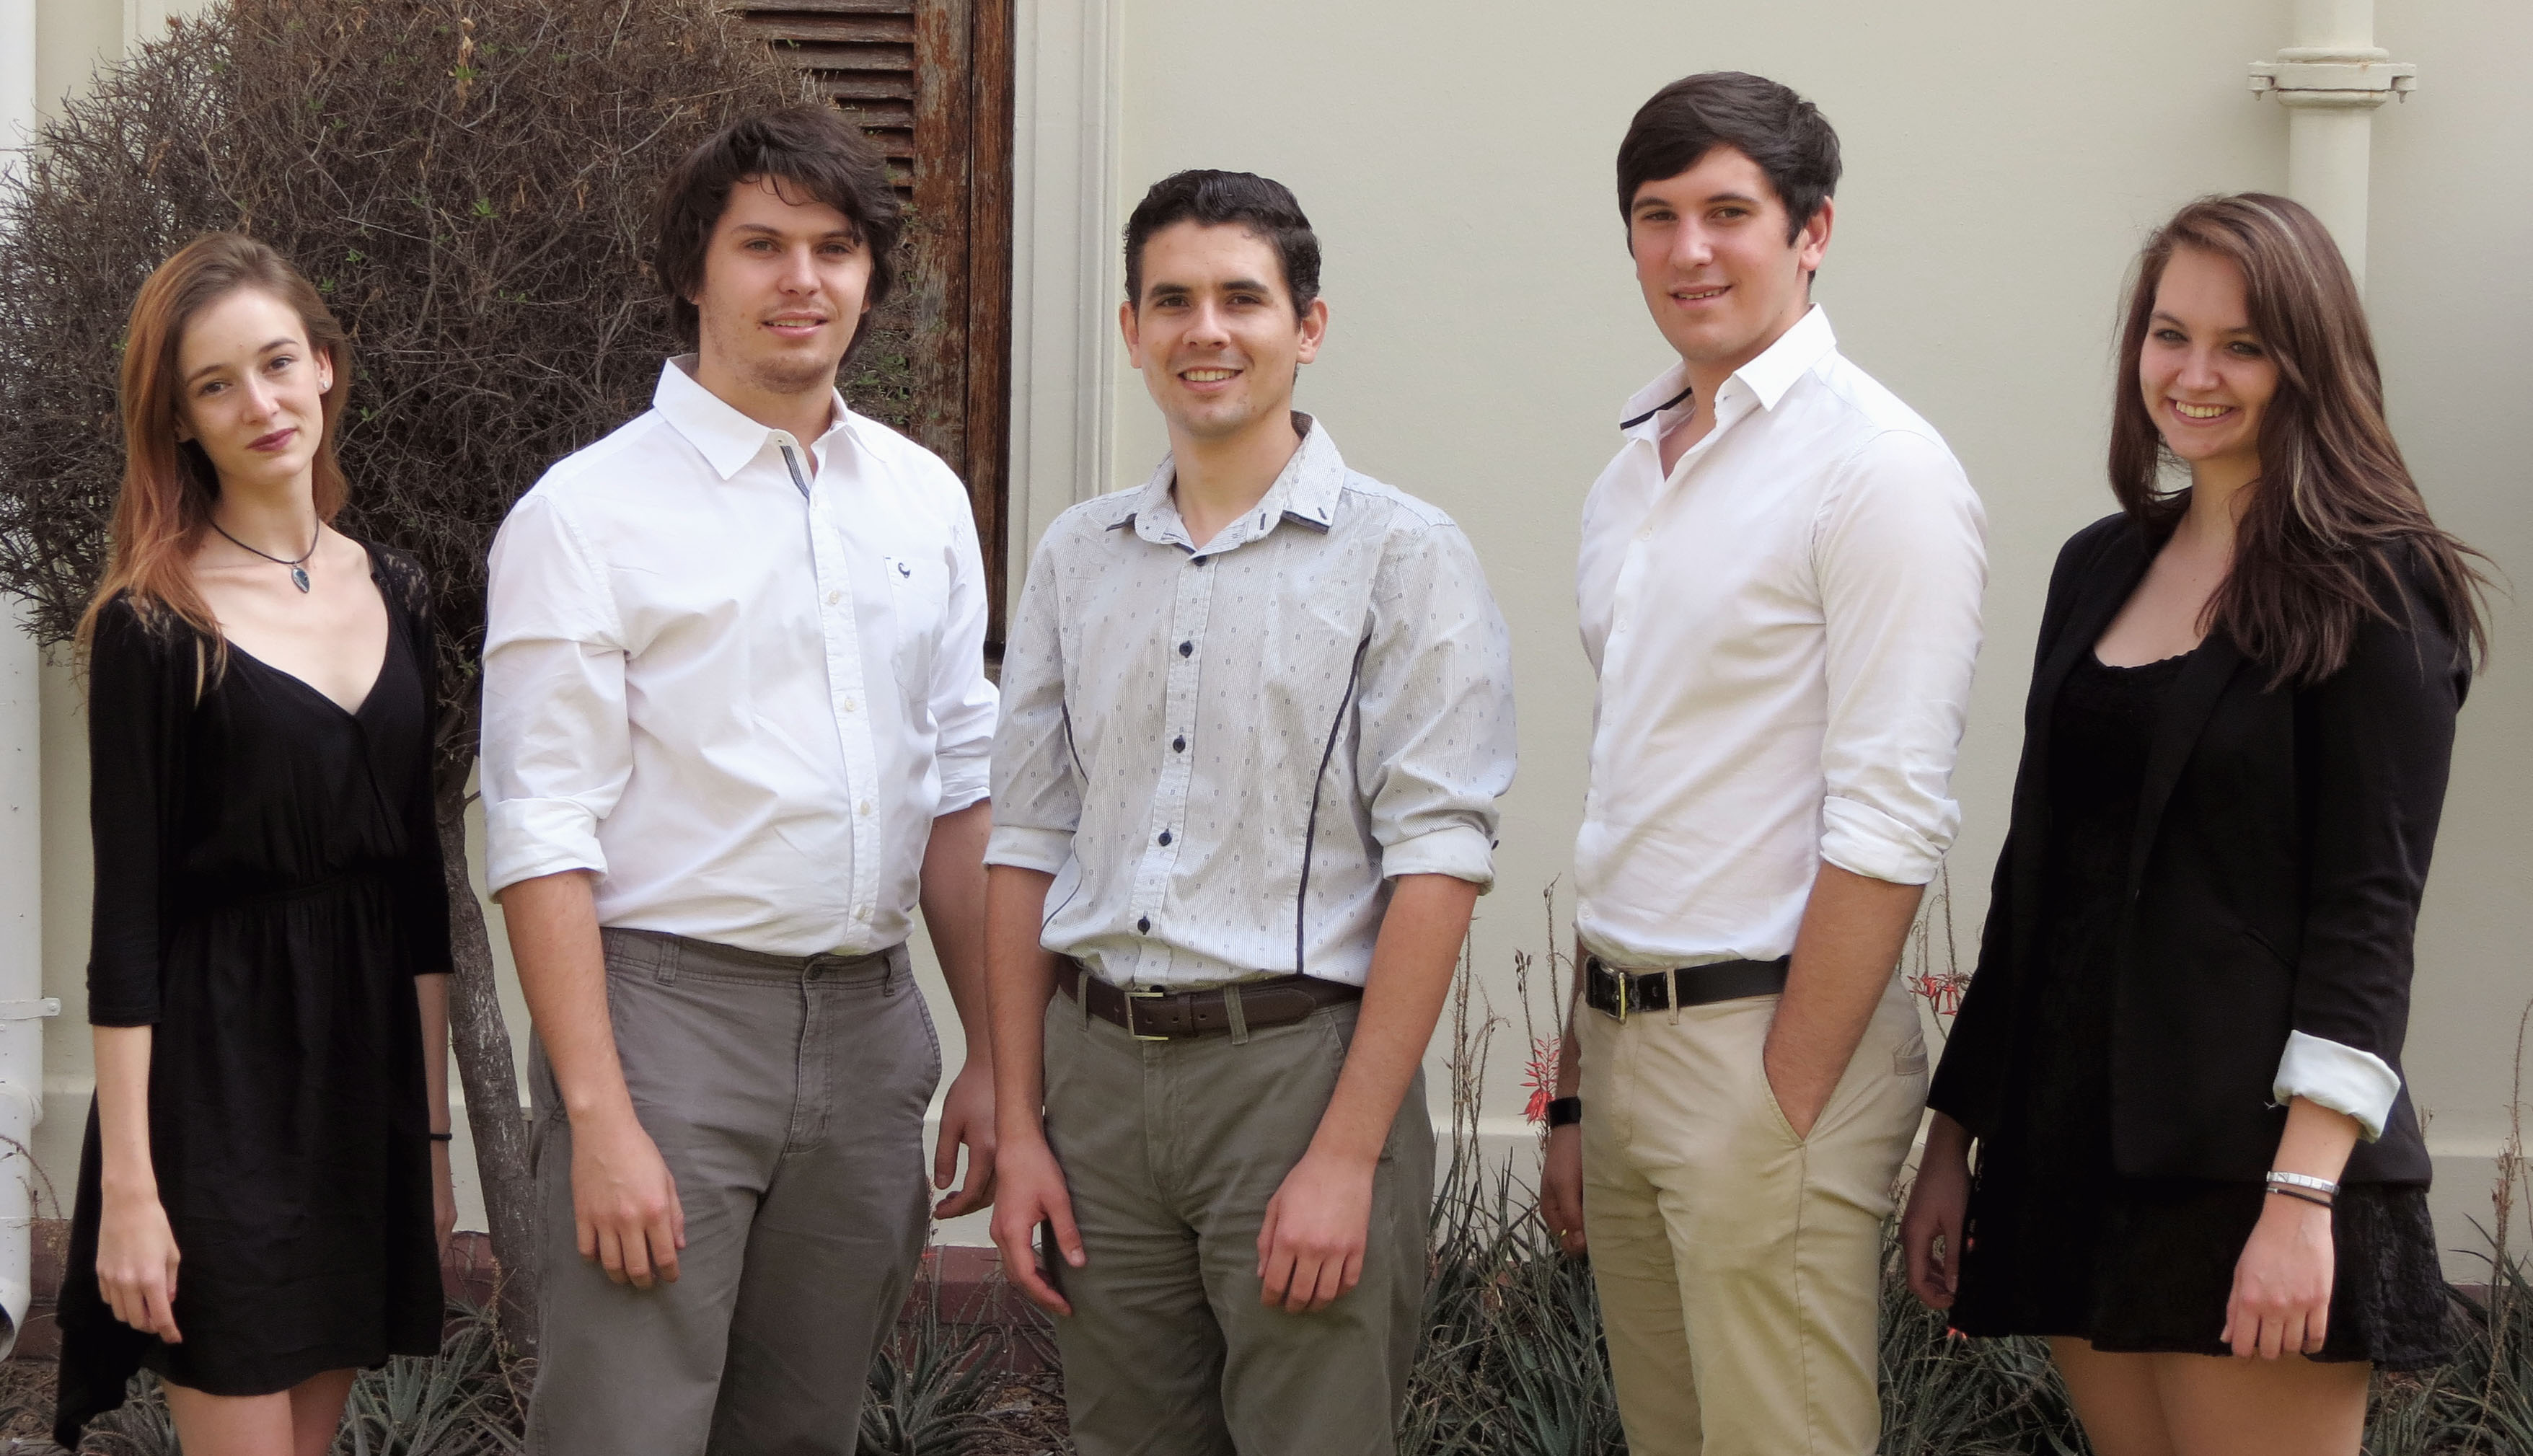
\includegraphics[width=0.9\textwidth]{team.jpg}};
            \node[fit=(pict),rounded corners=.55cm,inner sep=2pt]{};
         \end{tikzpicture}

         \par\vspace{1cm}
         \date{}
         \author{}
         \title{}
         \centering
         \textbf{Authors:}\\
         Mia Gerber\\
         Matthew Perry\\
         Wanrick Willemse\\
         Duart Breedt\\
         Linda Potgieter\\
      }
   \end{titlepage}
   \maketitle
   \tableofcontents
   \newpage
   
   \section{Project Description}
The project scope includes creating a RFID reader interface, storing timing and athlete data on a database when both online and offline, performing statistical analysis on database data, high Human Computer Interaction design standards when considering Graphical User Interface design, as well as successful registration of athletes.\\\\
The system will consist of technology to interface with the RFID reader provided by the client. We will only be able to decide on technology to interface with this reader when we have access to it. \\\\
Web Development technologies such as PHP, HTML, CSS, Bootstrap, JavaScript will be used to create a create a display that will be able to update in real time with data such as the current elapsed time and a number of athletes still participating. Any additional MEAN or LAMP stack technologies will be used as deemed necessary. The design of the web interface will be of utmost importance. The GUI will adhere to Human Computer Interaction Design principles to ensure effective use by the users.\\\\
For database functionalities, we will use SQL databases since there is no need for a great amount of handling of concurrent read and writes to the database. For Statistical analysis of the data, we will use math.js for calculations along with plot.js to visualise athlete relevant statistics based on the timing and distance data within the database. \\\\
We will design an interface which will be able to register an athlete to a specific RFID chip using a unique ID. Further registration specifics will depend on the design of the RFID and which data it can provide when read by the supplied reader.\\\\
When the RFID chip makes contact with the reader, data communication will be triggered. Details such as the athlete's unique ID and the exact time to finish the current race will be recorded and sent to either the online or the offline database. The unique ID is used in conjunction with the timing device data to ensure slow data transfer does not affect the recorded time.\\\\
A server will host this database to ensure real-time updating of the database. Server technologies will include MEAN Stack resources such as Node.js To ensure there is no data loss when there is no connection to the server (when the system is offline), data will be stored in a database. These data will then be uploaded to the database on the server as soon as there is an established connection between the two. As soon as the data are uploaded they will be removed from the offline database to prevent it from using unnecessary space. 


\subsection{Deployment Diagram}
\begin{center}
    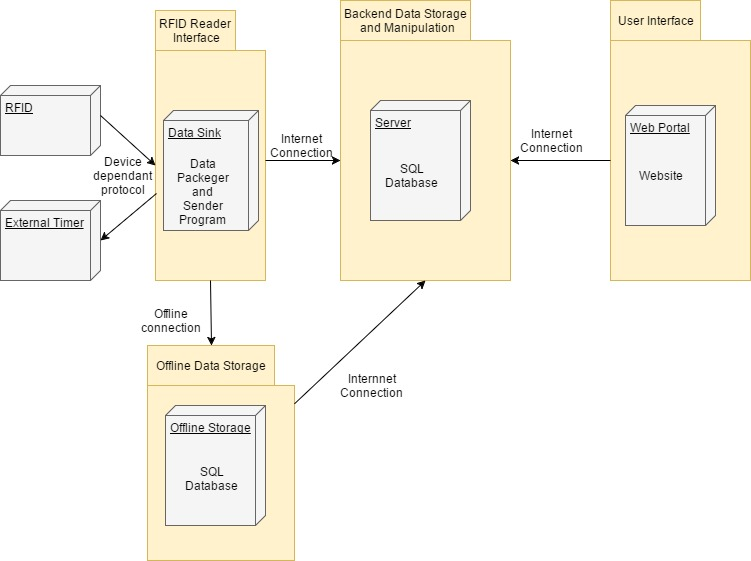
\includegraphics[width=0.5\linewidth]{ETADeployment.jpg}
\end{center}

\section{Development Methodologies}
\subsection{Interaction between development team and client}

\textnormal 
Involvement of the client is of utmost importance to ensure complete and on goal developed software. Client meetings will be arranged in advance with members of the team prepared with concerns and questions to ensure effective use of the client's time. 
As specified in the original project specifications provided by the client, the team will meet with the client either one week before, or one week after each major demonstration (dates of demonstrations as provided by the University of Pretoria COS 301 module). 
            \\ \\
            Moving more into the realm of software engineering, as a team we plan on strictly adhering 
            to Agile Principles. Clients will not only be queried for information but involved as much
            as possible in the testing of early prototypes so that their feedback can be integrated and 
            used as a guide for future releases.
            \\ \\
            Lastly, it is important to us that we as developers and you as our client at CSIR both 
            agree on a scope for the project, requirements can and probably will change but in order
            to provide the best quality product in the time-frame given we need to first create a checklist of features to be implemented and continually refer back to them to ensure we are not going off the scope.
                

\subsection{Interaction between members of development team}

\textnormal We decided on applying a SCRUM methodology in order to structure how teamwork will occur for
            this project, this is a faster, more intensely iterative approach to controlling workflow.
            We are using Slack and ZenHub (in conjunction with Github) to ensure that team members are aware of each other even when we are not physically together and are alerted when work is either available or completed.
            \\ \\
            Meetings will be held once a week regardless of whether there is a problem with the project or not, each meeting will require that each team member gives a small summary of what work they had done that week, this enforces accountability. Working in weekly "sprints" also optimises predictability and minimises risk (if something does go wrong it is only a week's worth of work lost, not a whole month)
            \\ \\
            As a team, we are going to be adhering to a practice called "pair-programming" which is essentially two or more people working on the same piece of code or feature in order to maximise the chances of bugs being discovered and minimise the time required to get a feature ready for production. \\\\
We will strictly follow the software development life cycle. 
Planning includes requirement and quality assurance analysis.   
The basic requirements have been provided, we have in this document defined and elaborated on them and their technologies. The client must approve these requirements and technologies.  \\\\
Once the client has given approval, we will start with designing the product architecture based on the requirements. This will clearly define all the architectural modules as well as its communication and data flow representation with the external and third party modules such as the external timing device and the RFID tags.  \\\\
After the design is complete, we will start with building the product using the agile methodology mentioned above. 
Testing will not be a once off phase, but instead, there will be continuous assessment of the product throughout the building process. Client input will be required for certain critical tests. \\\\
When the product is complete and complies with the team's high standards, it will be handed over to the CSIR for deployment. 
            \\ \\ 

    \newpage
    \section{Our Team}
              \parbox[c][4cm]{4cm}{\tikz\node[circle,draw,minimum size=3.5cm, 
			path picture={
               \node at (path picture bounding box.center){
                   
\includegraphics[width=3.5cm]{mia.jpg}
               };
           }]{};
		}
		\parbox[c][4cm]{10cm}{\subsection*{Mia Gerber}B.IS Multimedia}\\\\
Logical thinking and reasoning has always come naturally to me, I enjoy being posed a question or problem and then left to use the tools at my disposal to answer and/or solve it.\\\\
I am stubborn in the pursuit of success, which leads to many hours being sunk into troubleshooting if a product or deliverable does not meet all the requirements.\\\\
I am skilled in both the technical and creative side of development, in other words, formulating somewhat unconventional solutions and then executing them in a professional manner.\\\\
I believe that my team members and I are capable of making this project a success through our already existing abilities as well as sheer tenacity.\\\\
		\textbf{\small Experience and Project:}\\
		University of Pretoria’s EBIT Week IT team\\
		eCommerce website (both front and backend development) as undergraduate project\\
		Teaching Assistant for the Computer Science department\\\\
		\parbox{\textwidth}{
			\textbf{\small Relevant skills:}
			\begin{itemize}\itemsep0em
				\item Programming Languages:
				\begin {itemize}\itemsep0em
					\item C++
					\item C
					\item C\#
					\item Java
					\item x86 Assembly Language
					\item Javascript
					\item JQuery
					\item Actionscript 3.0
				\end {itemize}
				\item Markup Languages:
				\begin {itemize}\itemsep0em
					\item XML
					\item HTML
					\item JSON
					\item CSS
					\item Bootstrap
				\end {itemize}
				\item Frameworks:
				\begin {itemize}\itemsep0em
					\item MEAN stack development
					\begin {itemize}\itemsep0em
						\item Node.js
						\item Angular.js
						\item Express.js
						\item MongoDB
					\end {itemize}
					\item LAMP stack development
					\begin {itemize}\itemsep0em
						\item MySQL
						\item PostgreSQL
						\item PHP
					\end {itemize}
				\end {itemize}
				\item Software:
				\begin {itemize}\itemsep0em
					\item Adobe Creative Suite
					\item Modelio
				\end {itemize}
			\end{itemize}
		}
		\newpage
		\parbox[c][4cm]{4cm}{\tikz\node[circle,draw,minimum size=3.5cm, 
			path picture={
               \node at (path picture bounding box.center){
                   
\includegraphics[width=3.5cm]{matthew.jpg}
               };
           }]{};
		}
		\parbox[c][4cm]{10cm}{\subsection*{Matthew Perry}B.Sc IT GIS}\\\\
		I am passionate about software development. Being able to write code to solve a problem excites me. I am driven to be able to learn new technologies and be able to use them to create software and solve problems. I am a critical thinker that thrives when given something complex to assess and work on.
I am able to work well under pressure and ensure that the final result exceeds expectations. I can adapt to the situation so that I can perform at my peak. Learning and gathering experience are very important aspects in my life.\\\\
		\textbf{\small Experience and Project:}\\
		HCI task to redesign an app to improve user experience.\\
		Programmed an FPGA board using VHDL.\\\\
		\parbox{\textwidth}{
			\textbf{\small Relevant skills:}\\
			\parbox{5cm}{
				\begin{itemize}\itemsep0em
					\item OOP
					\begin {itemize}\itemsep0em
						\item C++
						\item Java
						\item Python
						\item Javascript
					\end {itemize}
				\end {itemize}
			} 
			\parbox{5cm}{
				\begin{itemize}\itemsep0em	
					\item Web Development
					\begin {itemize}\itemsep0em
						\item HTML
						\item PHP
						\item NodeJS
						\item SQL
						\item MongoDB
					\end {itemize}
				\end {itemize}
			}
			\begin{itemize}\itemsep0em	
				\item C
				\item Android Studio
				\item Hardware Descriptive Language: VHDL
				\item Cisco CCNA 6.0 and CCNP Route qualifications
				\item GIS (ArcGIS, QGIS)
			\end{itemize}
		}
		\newpage
		\parbox[c][4cm]{4cm}{\tikz\node[circle,draw,minimum size=3.5cm, 
			path picture={
               \node at (path picture bounding box.center){
                   
\includegraphics[width=3.5cm]{wanrick.jpg}
               };
           }]{};
		}
		\parbox[c][4cm]{10cm}{\subsection*{Wanrick Willemse}B.IS Multimedia}\\\\
		I’ve always enjoyed finding a solution to a challenge. I believe that anything can be overcome if it is approached systematically and with determination.\\\\
Meticulous design and thorough planning should be at the forefront of tackling a problem. I try to establish a vision and use it as a roadmap when creating something. I consider a product successful when I can see it is of a high standard.\\\\
I am adaptable and can function well under pressure. When it comes to my work, there is no settling for second best.\\\\
Developing high-quality software expects no less.\\\\
		\textbf{\small Experience and Project:}\\
		7 years work experience at a pathology company\\
		eCommerce website as undergraduate project\\
		Tutor for first year webdesign and second year Visual Design\\\\
		\parbox{\textwidth}{
			\textbf{\small Relevant skills:}
			\begin{itemize}\itemsep0em
				\item OOP and Procedural programming in: C++, C, Java, PHP, Python and JavaScript
				\item Web Development: HTML, CSS, Bootstrap, MEAN and LAMP stack
				\item XML, JSON and WebGL
				\item Adobe Suite, HCI, UX and UI design
			\end{itemize}
		}
		\newpage
		\parbox[c][4cm]{4cm}{\tikz\node[circle,draw,minimum size=3.5cm, 
			path picture={
               \node at (path picture bounding box.center){
                   
\includegraphics[width=3.5cm]{duart.jpg}
               };
           }]{};
		}
		\parbox[c][4cm]{10cm}{\subsection*{Duart Breedt}B.IS Multimedia}\\\\
		I take pride in making all my work aesthetically pleasing and believe it is of the utmost importance that all user-centered products should have great UI and UX design.\\\\
I think of myself as a perfectionistic completionist. Characteristically, I work persistently on any endeavour I undertake until I have produced a quality product I am proud of.\\\\
\parbox{\textwidth}{I find that if I am not learning, I am bored. Therefore, I strive to seek out challenges which push my limits and force me to contend with steep learning curves.\\}
I strongly believe that if you ever wish to be great at what you do you should ensure you are never the smartest person in the room. People are vessels of knowledge and will teach you more than you would like to know if you let them.\\\\
		\textbf{\small Experience and Projects (Please see my LinkedIn and GitHub for more detail):}\\
		Developed a website for Caelum Technologies\\
		Developing a website for the National Field Trial Association\\
		Developing a website for TallTrees Learning Community\\
		\href{http://77-breedt.000webhostapp.com}{Developed an ecommerce website as an undergraduate based project}\\\\
		\parbox{\textwidth}{		
			\textbf{\small Relevant skills:}
			\begin{itemize}\itemsep0em
				\item Object-Oriented Programming
				\item Java
				\item C++
				\item XML
				\item JSON
				\item Web Development:
				\begin {itemize}\itemsep0em
					\item HTML
					\item CSS
					\item Bootstrap
					\item Javascript
					\item JQuery
					\item MEAN stack (NodeJS, MongoDB, AngularJS)
					\item LAMP stack (PHP, SQL)
				\end {itemize}
				\item Design principles (UI, UX, HCI)
				\item Visual Design
				\item Adobe Creative Suite

			\end{itemize}
		}
		\newpage
		\parbox[c][4cm]{4cm}{\tikz\node[circle,draw,minimum size=3.5cm, 
			path picture={
               \node at (path picture bounding box.center){
                   
\includegraphics[width=3.5cm]{linda.jpg}
               };
           }]{};
		}
		\parbox[c][4cm]{10cm}{\subsection*{Linda Potgieter}B.Sc IT Genetics}\\\\
		I am always up for a challenge. Nothing great is worth achieving by taking the easy way out.. I am always analyzing the problem to ensure I find the most effective but easiest to understand solution.\\\\
I am always willing to find a solution to a problem on my own, but I know when I need to ask for assistance. Struggling alone is not an option when project quality is at stake. Strong believer in the use and creation of complete and concise documentation for any project. \\\\
I perform well under pressure, but ensure the pressure placed on myself with regards to my studies is at minimum by setting milestones and achieving them within a set timeframe. No one likes sloppy last minute work, and clients deserve more than that, even if it is only a teaching assistant assessing the work.\\\\
		\textbf{\small Experience and Project:}\\
		Redesign of mobile application to comply with HCI standards as undergraduate project.\\\\
		\parbox{\textwidth}{
			\textbf{\small Relevant skills:}
			\begin{itemize}\itemsep0em
				\item Java
				\item Python
				\item C++
				\item x86 Assembly Language 
				\item JSON
				\item Web development
				\begin {itemize}\itemsep0em
					\item HTML
					\item CSS
					\item Bootstrap
					\item XML
					\item JavaScript
					\item JQuery
					\item MEAN Stack
					\begin {itemize}\itemsep0em
						\item AngularJS
						\item NodeJS
						\item MongoDB
						\item ExpressJS
					\end {itemize}
					\item LAMP stack
					\begin {itemize}\itemsep0em
						\item PHP
						\item SQL (MySQL and MSQL)
					\end {itemize}
				\end {itemize}
				\item Design principles
				\item Human Computer Interaction design
				\item User interface design
				\item User experience design
				\item Other 
				\begin {itemize}\itemsep0em
					\item Genome analysis programs 
					\begin {itemize}\itemsep0em
						\item MEGA 6.06
						\item Mothur
						\item MCRobot
					\end {itemize}
				\end {itemize}
			\end{itemize}
		}

\end{document}
